Filas de prioridades são estruturas de dados essenciais que permitem o armazenamento de elementos com a capacidade de recuperar rapidamente o item com a maior (ou menor) prioridade. Em um \textit{min-heap}, a prioridade é determinada pela chave do elemento, onde uma chave menor indica uma prioridade mais alta.

\subsection*{Operações Fundamentais}

\begin{itemize}
  \item \textbf{heap\_minimum}: Esta operação retorna o elemento com a menor chave no min-heap, que é sempre o elemento na raiz da árvore. Sua complexidade é $O(1)$, pois o elemento mínimo é acessado diretamente.
  
  \item \textbf{heap\_extract\_min}: Remove e retorna o elemento com a menor chave no min-heap. A complexidade desta operação é $O(\log n)$ devido ao processo de reestruturação do heap após a remoção do elemento mínimo.
  
  \item \textbf{heap\_increase\_key}: Aumenta o valor da chave de um elemento em um min-heap. Após o aumento, o heap é ajustado para manter a propriedade de min-heap, o que leva a uma complexidade de $O(\log n)$.
  
  \item \textbf{min\_heap\_insert}: Insere um novo elemento no min-heap. A inserção pode exigir a reestruturação do heap para manter a propriedade de ordenação, resultando em uma complexidade de $O(\log n)$.
\end{itemize}

Essas operações permitem que as filas de prioridades baseadas em min-heap ofereçam uma maneira eficiente de acessar e modificar elementos com base em suas prioridades, mantendo uma complexidade logarítmica para as operações mais custosas.

\begin{figure}[H]
    \centering
    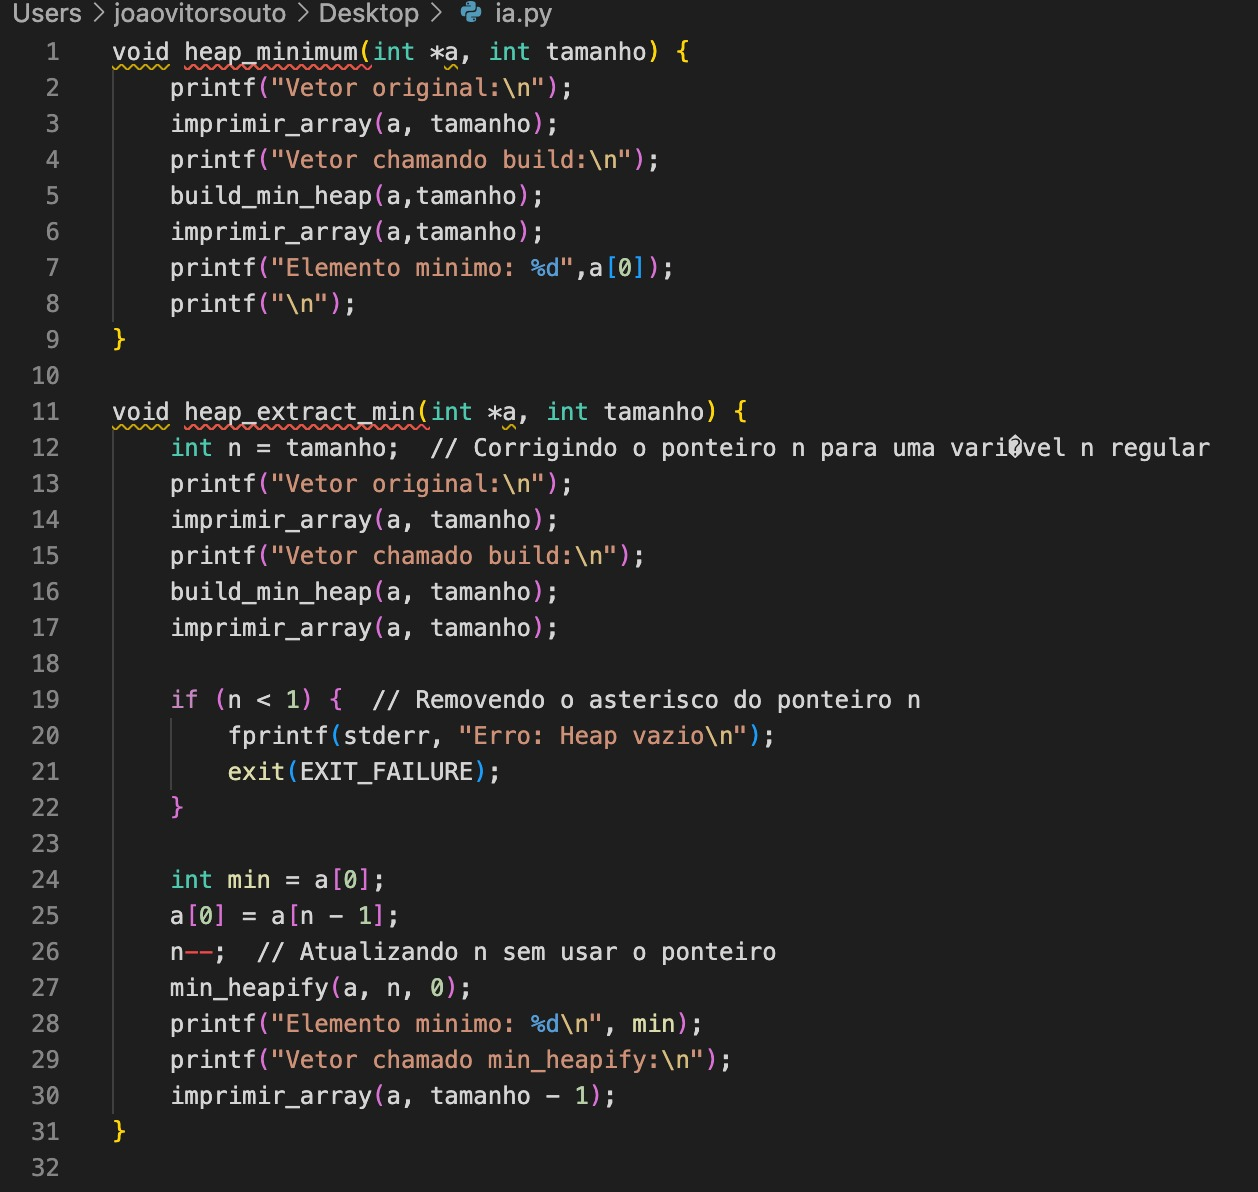
\includegraphics[width = 10cm]{Imagens/fila/98cf0803-8396-443a-a626-22850b4a8a54.jpg}
    \caption{Código Fila de Prioridade}
    \label{grafico_insert}
\end{figure}

\begin{figure}[H]
    \centering
    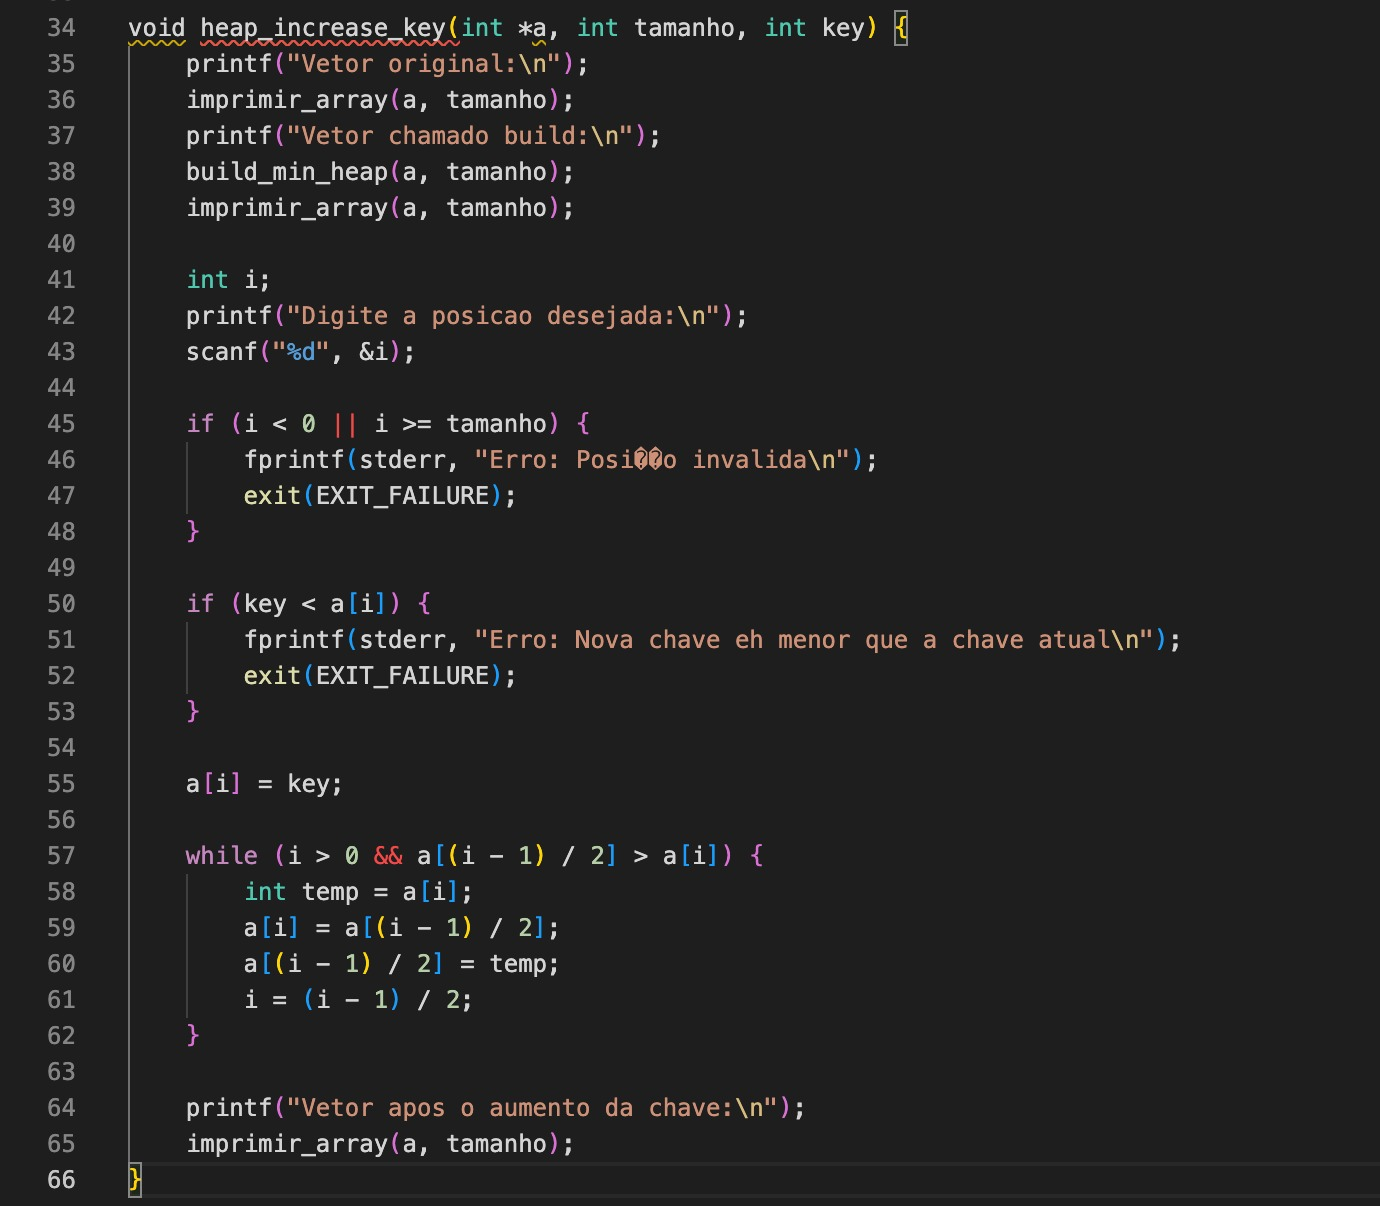
\includegraphics[width = 10cm]{Imagens/fila/5f8a8050-b74b-4d6d-8770-07522b37a09a.jpg}
    \caption{Código Fila de Prioridade 2}
    \label{grafico_insert}
\end{figure}